\newpage
\section{Suns-Jsc editor}
The Jsc editor can be used to configure suns-Jsc simulations. It enables you to set the start light intensity, stop light intensity and how big the steps are. This is shown in figure \ref{fig:sunsjsceditor}.

\begin{figure}[H]
\centering
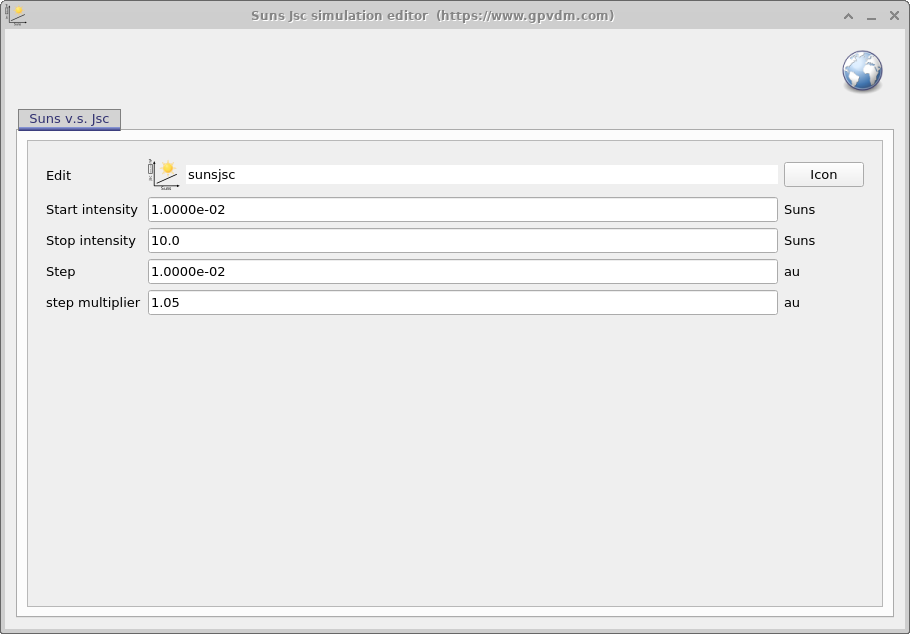
\includegraphics[width=0.7\textwidth,height=0.5\textwidth]{./images/sim_editors/suns_jsc_editor.png}
\caption{The JV curve editor window}
\label{fig:sunsjsceditor}
\end{figure}


\subsection{Outputs}

\begin{table}[H]
\begin{center}
\begin{tabular}{ |c|c| } 
 \hline
	File name 		& 	Description  \\ 
 \hline
	suns\_jsc.csv 	&	Suns v.s. Jsc curve \\ 
	suns\_mu.csv		&	Suns v.s. average charge carrier mobility \\ 
 \hline
\end{tabular}
\caption{Files produced by the Suns-Jsc simulation}
\label{tab:suns_jsc_output}
\end{center}
\end{table}
